\documentclass[conference]{IEEEtran}
%\IEEEoverridecommandlockouts
\usepackage{tabularx}
\usepackage{cite}
\usepackage{amsmath,amssymb,amsfonts}
\usepackage{algorithmic}
\usepackage{graphicx}
\usepackage{textcomp}
\usepackage{xcolor}
\usepackage{todonotes}
\usepackage{url}
\usepackage{microtype}
\usepackage{comment}
\usepackage[hidelinks]{hyperref}
\usepackage{flushend}
\usepackage{listings}
\renewcommand{\ttfamily}{\small\fontfamily{cmtt}\selectfont}
\usepackage{booktabs}
\usepackage{xspace}
\newcommand{\evosuite}{\textsc{EvoSuite}\@\xspace}
\newcommand{\tool}{\textsc{Tool}\@\xspace}
\usepackage{xcolor}
\usepackage{pifont}

\newcommand{\valerio}[1]{\textbf{\textcolor{blue}{[ \ding{46}Valerio: #1]}}}
\newcommand{\jens}[1]{\textbf{\textcolor{magenta}{[ \ding{46}Jens: #1]}}}
\newcommand{\tim}[1]{\textbf{\textcolor{violet}{[ \ding{46}Tim: #1]}}}
\newcommand{\behnaz}[1]
{\textbf{\textcolor{teal}{[ \ding{46}Behnaz: #1]}}}
\newcommand{\inputgen}[1]{\input{generated/#1}\unskip}

%% Temporarily turn off TODOs
%\renewcommand{\valerio}[1]{}
%\renewcommand{\jens}[1]{}
%\renewcommand{\tim}[1]{}
%\renewcommand{\behnaz}[1]{}

\lstdefinestyle{mystyle}{
	numberstyle=\tiny,
	basicstyle=\ttfamily\footnotesize,
	breakatwhitespace=false,         
	breaklines=true,                 
	captionpos=b,                    
	keepspaces=true,                 
	numbers=left,                    
	numbersep=5pt,                  
	showspaces=false,                
	showstringspaces=false,
	showtabs=false,                  
	tabsize=2,
	frame=single
}

\lstset{style=mystyle}


\begin{document}

\title{Towards Cross-Build Differential Testing}

%\thanks{Identify applicable funding agency here. If none, delete this.}
% Valerio: this is for the camera ready version

%\author{Anonymous Author(s)}
%Valerio: the track is double blind

\author{\IEEEauthorblockN{1\textsuperscript{st} Jens Dietrich  \hspace{1cm} 2\textsuperscript{nd} Tim White}
\IEEEauthorblockA{\textit{Victoria University of Wellington} \\
Wellington, New Zealand \\
\{jens.dietrich,tim.white\}@vuw.ac.nz}
\and
\IEEEauthorblockN{3\textsuperscript{rd} Valerio Terragni}
\IEEEauthorblockA{\textit{University of Auckland} \\
Auckland, New Zealand \\
v.terragni@auckland.ac.nz}
\and
\IEEEauthorblockN{4\textsuperscript{th} Behnaz Hassanshahi}
\IEEEauthorblockA{\textit{Oracle Labs Australia} \\
Brisbane, Australia \\
behnaz.hassanshahi@oracle.com}
}


\maketitle

\begin{abstract}
%\valerio{For the terminology we need to be a bit careful, if we are assuming that one of the jar we are comparing is correct, then is regression testing, otherwise if we are not making any assumption of what jar version is correct but we are just exposing behavioural differences than we are doing differential testing. Are we assuming that the jars in Maven Central are the correct ones ?  }

Recent concerns about software supply chain security  have led to the emergence of different binaries built from the same source code. This will sometimes result in binaries that are not identical and therefore have  different cryptographic hashes. The question arises whether those binaries are still  equivalent, i.e., whether they have the same behaviour.  We explore whether differential testing can be used to provide evidence for non-equivalence.

We study this for \inputgen{num-pairs-of-binaries} pairs of binaries built for the same Maven artifact version,  distributed on Maven Central, Google Assured Open Source Software and/or Oracle Build-From-Source. We use \evosuite to generate tests for the baseline binary from Maven Central, run these tests against  this baseline binary and any available alternately built binaries, and compare the results for consistency. We argue that any differences may indicate variations in program behaviour and could, therefore, be used to detect compromised binaries or failures at runtime.

% We find a few cases where the test results show inconsistencies. Those cases can be attributed to errors in the configuration of reproducible builds and shortcomings of the current version of \evosuite. 

%While we did not detect any compromised builds in our experiments, our approach successfully identified two build configuration errors that led to changes in runtime behaviour, highlighting areas for improvement.
Although our preliminary experiments did not reveal any compromised builds, our approach successfully identified three build configuration errors that caused changes in runtime behaviour. These findings underscore the potential of our method to uncover subtle build differences, highlighting opportunities for improvement.

%The purpose of generating differential tests is to detect behaviour differences between different programs.   therefore safeguarding against the introduction of bugs, and detecting changes that may break  clients downstream. We explore a different use case for regression testing – to detect behaviour changes  between different builds of the same version. This is motivated by concerns about software supply chain security that have led to the emergence of different binaries built from the same source code. We study this for \inputgen{num-pairs-of-binaries} pairs of binaries built from the same source distributed using Maven Central, Google Assured Open Source Software and Oracle Build-From-Source. 
%We find that ..

\end{abstract}

\begin{IEEEkeywords}
test generation, differential testing, reproducible builds, software supply chain security, java, evosuite
\end{IEEEkeywords}

\section{Introduction}

Software supply chain security has attracted increasing attention recently after a number of high impact attacks such as \textsf{equifax}, \textsf{log4shell}, \textsf{solarwinds} and \textsf{xz}~\cite{ellison2010evaluating,martinez2021software,enck2022top,EO14028}. In general, these fall into two categories -- compromising components (such as \textsf{equifax} and \textsf{log4shell}), and compromising processes (such as \textsf{solarwinds} and \textsf{xz}). When build processes are compromised, attackers can inject malicious code into a program, resulting in a vulnerable program built from clean source code. The classic approach to achieve this is to compromise the compiler~\cite{thompson1984reflections}. 

Reproducible builds~\cite{reproduciblebuild, lamb2021reproducible} are a common countermeasure. The idea is to perform a second build leading to the same binary. As an adversary is very unlikely to compromise two build environments, this can confirm the integrity of the binary with high certainty. Establishing that the binaries are identical is usually done by means of bitwise comparison, often using cryptographic hashes as proxies.
Several organisations have started to provide infrastructure and services to provide such secondary builds at scale, often meeting additional security-related requirements, such as SLSA compliance~\cite{slsa}. Two such products that include support to build Java / Maven artifacts are Google's \textit{Assured Open Source Software (gaoss)}\footnote{\url{https://cloud.google.com/security/products/assured-open-source-software}}, and Oracle's \textit{Build-From-Source (obfs})\footnote{\url{https://maven.oracle.com/public/}}.

However, there are several challenges with the reproducibility of builds: (i) build environments are difficult to replicate, (ii) locating the source code version (commit, tag or release) associated with a binary release version is not always straightforward and (iii) builds may be non-deterministic~\cite{xiong2022towards,hassanshahi2023macaron,bineqdataset,keshani2024aroma}. In particular, different versions of compilers may employ different compilation strategies, resulting in different, yet functionally equivalent binaries~\cite{xiong2022towards,bineqdataset,schott2024JNorm}.  
In order to address this, bytecode normalisation techniques have recently been proposed~\cite{xiong2022towards,dietrich2024levelsbinaryequivalencecomparison,schott2024JNorm}. 

From a security analysis perspective, comparing binaries from alternative builds can help detect potential compromises. If two binaries differ, it may indicate that one has been compromised, potentially by the insertion of a backdoor during the build process. A comparison based on strict binary equality is likely to result in poor precision as differences between binaries can be explained by the variability of compilers and other tools used in the build toolchain. Low precision is known to have a serious impact on the acceptance of program analysis tools by engineers~\cite{sadowski2018lessons,distefano2019scaling}. Using bytecode normalisation techniques such as \textit{jnorm}~\cite{schott2024JNorm} can help to reduce the false positive rate by identifying \textit{equivalent} binaries. The question arises whether binaries built from the same sources that are not equivalent actually have behavioural differences. A good way to check this is to find or construct test cases to demonstrate such differences.

%\valerio{I think we should frame this paper as Emerging Results paper following the call for papers. what do you think ? We should not present it as a study, but we should focus on the idea itself}
%\tim{Valerio, it looks like the 2 categories for short papers call for papers are:
%	\begin{enumerate}
%		\item Groundbreaking research papers: Exciting new directions or techniques that may have yet to be supported by solid experimental results but supported by strong and well-argued scientific intuitions.
%		\item Reflection papers: Bold and unexpected results and reflections that challenge the existing research outcomes and help us look at current research directions in a new light, calling for fundamentally new future research directions.
%	\end{enumerate}
%	Which are you thinking is more suitable? I'm thinking ``reflection paper''.
%}
This is the question we set out to study. We use test case generation with \evosuite~\cite{fraser2011evosuite} to synthesise regression tests for a baseline build, and then assess whether these tests behave in the same way on programs that are the result of an alternative  build from the same sources. 

% Jens: can drop this if we need space
The paper is organised as follows: in Section~\ref{sec:methodology} we describe the methodology used in our study.  Results are discussed in Section~\ref{sec:results}, followed by a brief overview of related work in Section~\ref{sec:relatedwork} and the conclusion (Section~\ref{sec:conclusion}). Details on how to access the dataset used and the generated tests are provided in Section~\ref{sec:dataaccess}. 

\section{Methodology}
\label{sec:methodology}


\subsection{Overview}

An overview of our methodology is depicted in Figure~\ref{fig:methodology}.  As a baseline build we use the artifacts distributed on Maven Central\footnote{\url{https://central.sonatype.com/}} as this is the default artifact repository for most open source Java projects.  From there we obtain the binary (jar file containing Java bytecode) \textit{mvnc jar} and the pom \textit{mvnc pom}. From this pom we extract the \textit{dependencies} using the Maven dependency plugin\footnote{\url{https://maven.apache.org/plugins/maven-dependency-plugin/}}. The \textit{mvnc jar} and its \textit{dependencies} can be used as input to generate \textit{test sources} with \evosuite, which are then compiled into test binaries (\textit{test bin}). Finally, these tests can be executed against both the original \textit{mvnc jar} and an alternative jar (\textit{alt jar}) from a different build, with the resulting test reports compared.

\begin{figure}[t!]
	\centering
	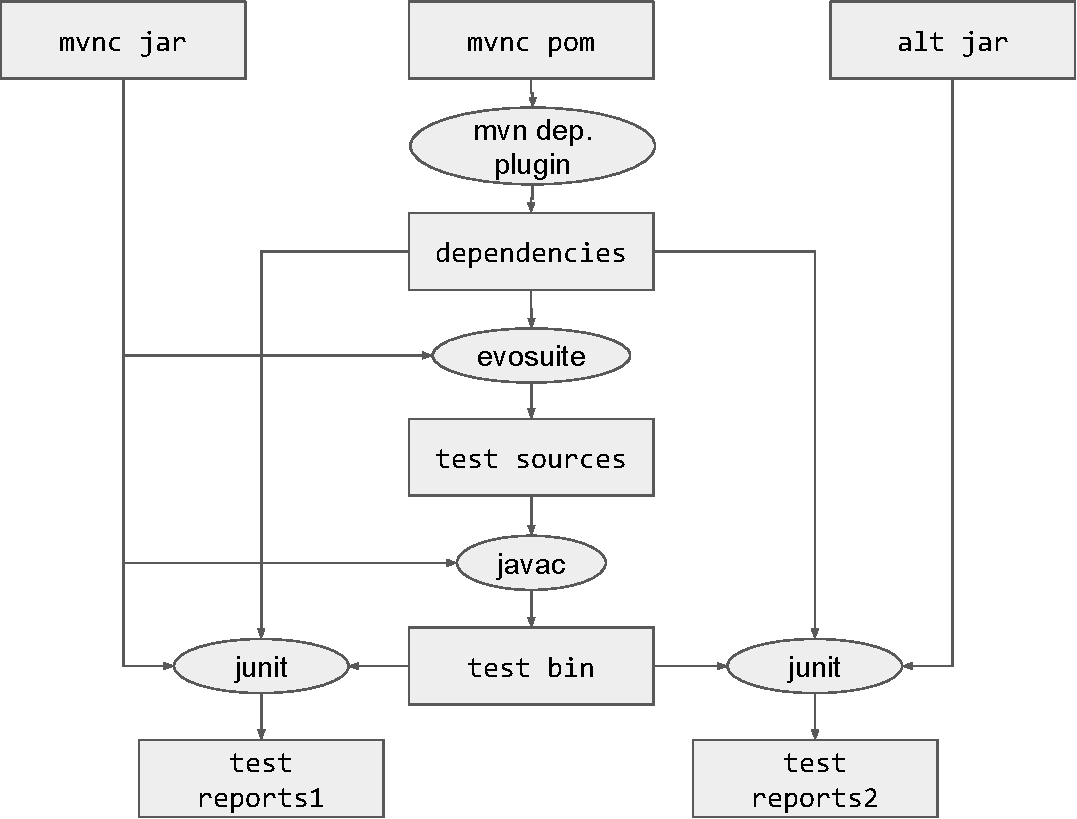
\includegraphics[width=\columnwidth]{figures/methodology.pdf}
	\caption{Methodology Overview \label{fig:methodology}}
\end{figure}


\subsection{Project Selection}

We started with the dataset from Dietrich et al.~\cite{dietrich2024levelsbinaryequivalencecomparison}, which contains jars corresponding to the same artifact identified by the same group id, artifact id and version (i.e., GAV coordinates) built by different parties. This dataset contains the results of builds from Maven Central (\textit{mvnc}), Google (\textit{gaoss}), Oracle (\textit{obfs}) and  RedHat. We ignored jars built by RedHat as they have an additional patch id that suggests behavioural differences.  We only considered pairs where one of the jars was sourced from Maven Central, i.e., built by the developer(s). There are \inputgen{num-pairs-of-binaries} such pairs.


\subsection{Static Pre-analysis}

We then ran a static pre-analysis to eliminate pairs that are probably equivalent. We first applied \textit{jnorm}~\cite{schott2024JNorm}\footnote{We used \textit{jnorm} version 1.0.0, downloaded from \url{https://github.com/stschott/jnorm-tool/releases/tag/v1.0.0}, with the arguments \texttt{-o -n -s -a -p}.}, and compared jars by comparing the result of the transformation applied to each class; we eliminated pairs with equal \textit{jnorm} output, resulting in \inputgen{num-jar-pairs-after-jnorm2} pairs of jars. We then applied a filter based on a change in the Java 18 compiler\footnote{\url{https://github.com/openjdk/jdk/pull/5165}}, which is not yet supported by \textit{jnorm}. Applying this additional filtering resulted in \inputgen{num-jar-pairs-after-invokevirtual-invokeinterface} pairs of jars, \inputgen{num-jar-pairs-after-invokevirtual-invokeinterface-gaoss} of those pairs with an alternatively built jar from \textit{gaoss}, \inputgen{num-jar-pairs-after-invokevirtual-invokeinterface-obfs} with such a jar from \textit{obfs}.
In total there are \inputgen{num-class-pairs-after-invokevirtual-invokeinterface} classes that differ between \textit{mvnc} and one of the other two providers, which reduces to \inputgen{num-top-level-class-pairs-after-invokevirtual-invokeinterface} after condensing classes to top-level classes.



\subsection{Test Generation}

We chose to automatically generate tests for these experiments because the existing tests within the project are typically executed during builds. In other words, alternative builds can ensure that such existing tests pass successfully.

We used \evosuite\footnote{\evosuite version 1.2.0, downloaded from \url{https://github.com/EvoSuite/evosuite/releases/tag/v1.2.0}}
to generate differential tests. Although various alternatives exist for Java test generation, recent benchmarks demonstrate \evosuite's superior performance in achieving higher code coverage and mutation scores~\cite{jahangirova2023sbft}.

%\valerio{I added some background on evosuite and regression testing in general, not sure where we want to put this but I think is important to explain how \evosuite exposes the behavioural differences}
\evosuite automatically generates test cases for a given object-oriented class under test (CUT). A test case consists of (i) a method call sequence that instantiates and modifies the state of objects of the CUT through method invocations and (ii) one or more assertions that predicate on the values returned by the method invocations. The state of objects often dictates program behaviour, so manipulating these states is crucial for achieving high coverage. It is worth noting that \evosuite may need to create and modify objects that do not instantiate the CUT, as the methods of the CUT might require non-primitive parameters. For primitive parameters, \evosuite uses randomised values guided by heuristics. The tool implements an evolutionary algorithm that evolves populations of test cases to maximise code coverage, typically targeting branch coverage.

\evosuite and similar automated testing tools are most effective when running in regression mode due to the oracle problem. In fact, they are predominantly evaluated in this mode~\cite{jahangirova2023sbft,shamshiri2015automatically}. While the oracle problem is one of the greatest challenges in test automation, it is mitigated in the context of regression testing, where we assume that one version is correct. In regression mode, \evosuite adds assertions to the generated test cases that capture the ``implemented'' behaviour of the given version. These assertions are based on the actual values returned by method call invocations during execution, without regard for the ``intended'' behaviour of the CUT. This approach also enables effective differential testing by identifying behavioural differences between two implementations (without assuming that one is correct). If a test generated for one version fails when run on another, it reveals a behavioural difference. % between the two versions.

\evosuite can be set up to generate targeted tests for certain classes. Since the static pre-analysis compares \textit{jar} files by comparing the \textit{.class} files they contain, we can use targeted test generation for those classes only.   
%Since the static pre-analysis compares JAR files via their \textit{.class} files, we generate tests only for those classes.

\evosuite was applied to generate regression tests for the \textit{mvnc} version of each of these \inputgen{num-top-level-class-pairs-after-invokevirtual-invokeinterface} differing top-level classes, resulting in \inputgen{num-classes-with-generated-tests} generated test classes comprising in total \inputgen{num-generated-tests} JUnit4 tests, or \inputgen{avg-tests-per-class} tests per differing class on average.

We ran \evosuite test generation per-class with all settings at their defaults, in particular with \texttt{search\_budget} (generation time) set to 1 minute.\footnote{Extending generation time to 10 minutes on a subset of classes did not generate any additional tests.}
All computation was performed using a JDK 8 toolchain on an 8-core Linux Mint 21.2 VM with 50GB RAM.\footnote{JDK 8 was used in order to improve the reliability of \evosuite test generation. Although \evosuite could sometimes generate tests under JDK 11---including for 32 CUTs that refused to compile at JDK 8---doing so produced around one third as many tests overall due to widespread failures.}
Resource settings were informed by \cite{jahangirova2023sbft}. 


\section{Results}
\label{sec:results}

\subsection{Overview}

Table~\ref{tab:data-summary} shows the number of differing test outcomes for each artifact where one or more tests produced a different outcome on an alternative build than on \textit{mvnc}.
Note that this excludes \inputgen{num-test-failures-on-mvnc} test failures that occurred on \textit{mvnc} itself.

\begin{table*}[h]
	\centering
    \caption{Number of tests with different results between \textit{mvnc} and alternative builds}
	\label{tab:data-summary}
	\inputgen{data-summary-table-tabular}
	
\end{table*}


We will now discuss the identified inconsistencies in detail.

\subsection{Incorrect Build Configurations}


The first kind of test outcome difference, corresponding to rows 4--11 of Table~\ref{tab:data-summary}, occurs 48 times across 7 versions of \texttt{io.undertow:undertow-servlet}, and twice ``in the other direction'' in \texttt{io.netty.netty-codec-http:4.1.102.Final}.
We first describe the \textit{undertow-servlet} cases.

For each of the 7 versions of the \textit{undertow-servlet} artifact shown in Table~\ref{tab:data-summary}, there are two binaries available: the jar from \textit{mvnc}, and an alternatively built jar from \textit{gaoss}. In each case, when the \textit{gaoss} jar is tested using the \texttt{io.under\-tow.\-servlet.\-spec.UpgradeServletInputStream\_ESTest}\footnote{The class under test by an \evosuite-generated test can easily be identified by removing the \textit{\_ESTest} suffix.} test class generated from the \textit{mvnc} jar, test failures occur, while these tests all succeed against the original \textit{mvnc} jar.

All 48 \textit{gaoss} test failures result from a \texttt{java.lang.NoSuchMethodError}, caused by an attempt to invoke \texttt{java.nio.ByteBuffer.flip()Ljava/nio/ByteBuffer;}.
Failure counts vary across versions only because of random variation in the number of test methods that (indirectly) attempt to call this method.
Concretely, for version \textit{2.2.23.Final}, the 5 failing tests are \textit{test00}, \textit{test01}, \textit{test12}, \textit{test15} and \textit{test16}.

The errors occur during linking, and are related to binary compatibility~\cite{JVM17Spec}: Two \textit{undertow} methods (\texttt{UpgradeServletInputStream.readIntoBufferNonBlocking} and \texttt{UpgradeServletInputStream.readIntoBuffer}) have call sites for this method, however, the method is missing. 
A closer inspection reveals that the \textit{gaoss} version was built with Java 11\footnote{The jar manifest contains the entry \textit{Build-Jdk-Spec: 11}}. In Java 11, \texttt{java.nio.\-ByteBuffer.flip()Ljava/nio/ByteBuffer;}~exists\footnote{Though its existence is not mentioned in the documentation at \url{https://docs.oracle.com/en/java/javase/11/docs/api/java.base/java/nio/ByteBuffer.html}.}, and the respective call site is added. The \textit{mvnc} jar was built against Java 8, where this method did not exist, causing the compiler to instead add a call site to invoke \texttt{java/\-nio/ByteBuffer.flip:()Ljava/nio/Buffer;}\footnote{Unlike Java source code, Java byte code supports return type overloading, and changing the return types alters the descriptor, and therefore is a binary incompatible change causing linkage errors.~\cite{JVM17Spec,dietrich2014broken}}.

Therefore, this issue is caused by the different JDK versions used during the build. This is surprising, as reproducing builds usually try to replicate the build environment in order to maximise the chances of the build to succeed and the resulting binary to be identical to the original binary. In this case the engineers seem to have attempted this somehow by setting the compiler target level to bytecode version 52, which is associated with Java 8~\cite[Sect. 4.1]{JVM17Spec} instead of using version 55 associated with Java 11.  However, they did not account for the fact that there are changes in the standard library that have an impact on how bytecode is compiled. Since Java 9 (JEP247~\cite{jep247}), there is a \textit{-release} compiler  flag that can be used to avoid issues like this. It is likely that engineers used only \textit{-target} instead. The generated tests reveal those changes.  

\begin{table}[h]
	\centering
    \caption{Test results for \textit{UpgradeServletInputStream\_ESTest} tests on \textit{io.undertow:undertow-servlet:2.2.23} and for \textit{io.netty.handler.codec.http.multipart.AbstractDiskHttpData\_ESTest} tests on \textit{io.netty.netty-codec-http:4.1.102.Final}, running tests on the original Maven Central artifact and the alternative build from \textit{gaoss}}
    
	\begin{tabular}{p{0.8cm}p{0.5cm}p{0.9cm}p{1.6cm}p{1.3cm}p{1.3cm}}
		\toprule
		\textbf{artifact} & \textbf{build}         & \textbf{bytecode version} & \textbf{JDK version used to build} & \textbf{test results (Java 8)}                                                    & \textbf{test results (Java 11)} \\ \midrule
		undertow & mvnc & 52               & 8                         & pass                                                                     & pass                   \\
		undertow & gaoss         & 52               & 11                        & fail & pass                  \\ \hline
		netty & mvnc & 52               & 19                         & pass                                                                     & fail                   \\
		netty & gaoss         & 50               & 8                        & fail & fail                  \\ \bottomrule
	\end{tabular}
	
	\label{tab:nosuchmethoderror}
\end{table}

The two \textit{gaoss} test failures on \texttt{io.netty.netty-\-codec-http:4.1.102.Final} are similar, but ``in reverse'': Here, it is the \textit{mvnc} jar that was built with a newer JDK version (19), while \textit{gaoss} was built with JDK 8\footnote{The jar manifests contain the entries \textit{Build-Jdk-Spec: 19} and \textit{Build-Jdk-Spec: 1.8}, respectively.}.
This time, the generated tests \textit{expect} \texttt{NoSuchMethodError} to be thrown, resulting in test failure on \textit{gaoss} when the call to \texttt{java/nio/ByteBuffer.flip:()Ljava/nio/Buffer;} completes normally.%
% Tim cutting this for space (and time):
%\footnote{Interestingly, the code paths that trigger the \textit{NoSuchMethodError} on \textit{mvnc} seem to occur only as a result of buggy interference between test methods: See \tim{add URL to anonymised description page, or cut} for details.}

Table~\ref{tab:nosuchmethoderror} summarises these findings. One might expect different behaviour not revealed by tests when tests are executed with Java 11, as the call sites in these two binaries refer to different methods in the standard libraries. However, this is not the case as the Java compiler creates a synthetic \textit{bridge method} when compiling overriding methods with covariant return types. In this case, it creates the bridge method \texttt{java.nio.ByteBuffer.flip()Ljava/nio/Buffer;}  that invokes \texttt{java.nio.ByteBuffer.flip()Ljava/nio/ByteBuffer;}. This bridge method is used during the  runtime resolution of the virtual call for the \textit{mvnc} binary.


\subsection{EvoSuite Mock Generation}


We have identified three generated test classes with inconsistent behaviour between the \textit{obfs} and \textit{mvnc} builds for \texttt{commons-io:commons-io:2.15.0}: 
\begin{enumerate}
	\item  \texttt{org...io.monitor.FileAlterationObserver\_ESTest}
    \item \texttt{org...io.filefilter.NotFileFilter\_ESTest}
    \item  \texttt{org...io.output.UncheckedAppendableImpl\_ESTest}
\end{enumerate}

All of these test inconsistencies are caused by the same pattern.  The \textit{obfs} binary was built  with Java 8, while the \textit{mvnc} binary was built with Java 21. The target level for both was set to 52 (compatible with Java 8). Table~\ref{tab:stackoverflow} summarises the situation.


\begin{table}[h]
\caption{Test results for selected tests generated for  \textit{commons-io:commons-io:2.15.0}, running tests on the original Maven Central artifact and the alternative build from \textit{obfs}}
	\centering
	\begin{tabular}{p{1.2cm}p{1.2cm}p{1.7cm}p{1.3cm}}
		\toprule
		\textbf{build}         & \textbf{bytecode version} & \textbf{JDK version used to build} & \textbf{test results (Java 8)  }                                          \\ \midrule
		mvnc & 52       & 21                        & pass                                                                                        \\
		obfs         & 52               & 8                        & fail              \\ \bottomrule
	\end{tabular}
	
	\label{tab:stackoverflow}
\end{table}

In Java 18, a subtle change occurred regarding how methods implemented in the root class (\texttt{java.lang.Object}) such as \texttt{toString}, \texttt{equals} and \texttt{hashCode} are invoked for interfaces\footnote{\url{https://github.com/openjdk/jdk/pull/5165}}.
For instance, consider the code in the following listing:

\begin{lstlisting}[language=Java]
Comparable comp =  ... ; 
comp.toString();
\end{lstlisting}	

Up to Java 17, this call was compiled to \texttt{invokevirtual Object::toString}\footnote{Package names and descriptors are omitted for brevity}. Starting with Java 18, this call is now compiled to \texttt{invokeinterface Comparable::toString}.

This results in changes to runtime behaviour when using the \evosuite runtime, as \evosuite replaces these calls with calls to its own mocks, such as  \texttt{org.evosuite.runtime.System::toString}. But this only replaces the older call pattern, not the new one. 

An example of such inconsistent behaviour we have encountered  is when a \texttt{toString} implementation is recursive. Then \evosuite generates a test with a self-referential data structure that expects a \texttt{StackOverFlowError} to occur when \texttt{toString} is invoked on this data structure. However, when the mock substitution is performed by \evosuite, this error does not occur as the mock \texttt{toString} method is not recursive, and the test fails. I.e., the test outcome now depends on whether \evosuite performs the substitution or not, and this depends on the compiler that had been used.

In this case we think the misconfiguration is on the Maven Central side, where a very recent Java version has been used to create a binary compatible with Java 8, but this hasn't been configured correctly.
%Tim: I would instead say it's a problem caused by EvoSuite not being maintained, but I know this is a delicate issue!





\section{Related Work}
\label{sec:relatedwork}

\emph{Differential Testing}\cite{difftesting} is an automated approach that identifies various errors by comparing the behaviour of two or more comparable systems\cite{xie2007towards,jin10:automated,diffgen}. In the context of object-oriented (OO) programming, notable techniques include \textsc{Diffut}\cite{xie2007towards}, \textsc{BeRT}\cite{jin10:automated}, and \textsc{DiffGen}~\cite{diffgen}. Similar to our approach, these techniques leverage the differences between two software versions to generate test cases that reveal behavioural discrepancies. However, our approach focuses on comparing binaries, which required us to design and implement specialised ad-hoc analyses.

Although the implementation details may differ, all differential testing techniques share the core idea of generating and executing the same test cases on the versions being compared to reveal behavioural differences. % One of the most common applications of differential testing is regression testing, where two versions of the same program are compared. 
While differential testing has been effective in detecting semantic errors in various domains (e.g., C compilers~\cite{Yang:compiler:pldi:2011} and JVM implementations~\cite{Chen:jvmdiff:pldi:2016}), to the best of our knowledge, it has not yet been applied to identify differences between alternative builds of the same program version.


\section{Data Access}
\label{sec:dataaccess}

The input jar pairs, generated tests and raw test run reports can be found here: \url{https://doi.org/10.5281/zenodo.14252188}.


\section{Conclusion}
\label{sec:conclusion}

In this paper we have explored a novel use case for differential testing: to assess the behavioural equivalence of binaries built independently from the same source code. Our research was motivated by software supply chain security. While we did not find any evidence that components in our dataset had been compromised during the build, we did find two interesting cases of build misconfiguration.  

A possible avenue for future research is to analyse other signals from test executions, namely coverage. This could still reveal differences in program behaviour not captured by the assertions in generated tests. 

\section*{Acknowledgements}

The work of the first two authors was supported by a gift by Oracle Labs Australia.

%\todo[inline] {tba after review \vspace{0.5cm}}

\bibliographystyle{plain}
\bibliography{references}

\end{document}
